\section{\texorpdfstring{The \Gls{spade}}{SPADe} flow revisited}
\label{sec:ch7_SPADeRevisited}
This section makes the \gls{spade} design flow (illustrated in Fig.~\ref{fig:ch7_ibc_overview} and introduced in Section \ref{sec:ch7_designFlow}) precise in the form of Algorithm~\ref{algo:SPADeFlow}, using the model transformations of Section~\ref{sec:ch7_ModelTransformations}. The model transformations are primarily used to construct implementation-aware graphs for workload and system scenarios. The integrated transformation from an \gls{ibc} graph to an implementation-aware graph is captured in Algorithm~\ref{algo:impAwGraph}.
Due to platform resource constraints (the total number of available cores $\numCoresAvailable$), design choices (number of pipes $\numPipes$, number of cores allocated per pipe $\numCoresParallel$), application characteristics, inter-frame dependencies (inter-frame dependence time $\fd$) and the possible camera frame-arrival period ($\fh$), the effective implementation can be: i) a non-pipelined implementation without parallelised sensing; ii) a non-pipelined implementation with parallelised sensing; iii) a pipelined implementation without parallelised sensing; and iv) a pipelined parallelism implementation. Section~\ref{sec:ch7_ImpAwGrTrans} explains Algorithm~\ref{algo:impAwGraph} for constructing implementation-aware graphs.
Section~\ref{sec:ch7_unified SPADe flow} elaborates \gls{spade} in Algorithm~\ref{algo:SPADeFlow}. We then explain the refinements for non-pipelined and pipelined implementations in Sections~\ref{sec:ch7_NEW_SPADeNP} and~\ref{sec:ch7_NEW_SPADe_pipelined}. 
The differentiation between non-pipelined and pipelined implementation is mainly needed for control design and switching. 
Further, we also explain the challenge due to inter-frame dependencies in a pipelined implementation in Section~\ref{sec:ch7_IFD}.

\begin{algorithm}
\SetAlgoLined
\SetKwInOut{Input}{input}\SetKwInOut{Output}{output}
\Input{$\SDFG,\ \tau,\ h,\ \actorET_{{\taskC}{\taskA}},\ \numPipes,\ \mathit{IFD}$ (the set of known inter-frame dependencies)}
\Output{Implementation-aware graph $\SDFG_{I}$}
$\SDFG_{1}=\transformFixTiming(\SDFG,\text{delay},(\numPipes\times h-\tau))$;~\label{algoStep:G1}\\
$\SDFG_{3}=\transformCamera(\transformReplicate(\SDFG_{1},\numPipes),\numPipes)$;~\label{algoStep:G3}\\
$\SDFG_{31}=\transformFixTiming(\SDFG_{3},\text{camera},h)$~\label{algoStep:G31}\\
\If{$\numPipes>1$, i.e. pipelining is allowed~\label{algoStep:if_p>1_IFD}}{
\ForEach{$(a,b)\in\mathit{IFD}$~\label{algoStep:IFDforloop}}{
$\SDFG_{31}=\transformIFD(\SDFG_{31},a,b,\numPipes);$
}
}
$\SDFG_{4}=\transformWorkload(\SDFG_{31},\numPipes)$;~\label{algoStep:G4}\\
$\SDFG_{I}=\transformFixTiming(\SDFG_{4},T_j,(\tau-\actorET_{{\taskC}{\taskA}})),\ 1\le j\le \numPipes$;~\label{algoStep:impAwGraph}\\
\caption{impAwGrTrans($\SDFG,\tau,h, \actorET_{{\taskC}{\taskA}},\numPipes)$}\label{algo:impAwGraph}
\end{algorithm}

\subsection{Implementation-aware graph transformation}
\label{sec:ch7_ImpAwGrTrans}
In this section, we explain the steps needed to obtain the implementation-aware graph of a workload or system scenario and formalise those in Algorithm~\ref{algo:impAwGraph}. The \textbf{input} \gls{sdfg} is the \gls{sdfg} of a single parallelised pipe of a single scenario, obtained after applying the $\transformSequential$ transformation (as explained in Section~\ref{sec:ch7_ModelTransformations}), as illustrated in Fig. \ref{fig:ch7_transformations}.
The other inputs to the algorithm are the delay $\tau$, period $h$, the total execution time of the control compute and actuation tasks $\actorET_{{\taskC}{\taskA}}$, and the number of pipes $\numPipes$.
Also, we assume that if there exist inter-frame dependencies, they are known as a subset of actors $\mathit{IFD},\ \mathit{IFD} \subseteq \Actors^2$.
An ordered pair of actors $(a,b)\in \mathit{IFD}$ models the inter-frame dependency between the actors $a$ and $b$.
The \textbf{output} of the algorithm is the implementation-aware graph $\SDFG_I$.

\textbf{Step~\ref{algoStep:G1}} ensures that we can achieve a constant sensor-to-actuator delay during mapping by assigning the execution time of the delay actor as $\numPipes\times h - \tau$ in $\SDFG$ to obtain $\SDFG_{1}$.
The delay actor fills up the time between when the actuation task (modelled by actor \taskA) finishes its execution until the completion of one pipe (see Fig.~\ref{fig:ch7_transformations}).
This ensures that each parallelised pipe, when mapped to the platform, can periodically execute with the period $\numPipes\times h$ and has a constant delay of $\tau$.
If we have $\numPipes$ pipes, we can ensure that the effective control sampling period is $h$.
\textbf{Step~\ref{algoStep:G3}} replicates the single parallelised pipe model $\SDFG_{1}$ $\numPipes$ times to model the pipelined execution and then adds camera-awareness to the graph $\SDFG_{1}$ as explained in Section~\ref{sec:ch7_ModelTransformations}.
\textbf{Step~\ref{algoStep:G31}} updates the execution time of the camera actor in line with the sampling period $h$.
Our model has to execute with the period $h$ even though the camera frame arrival period is $\fh$.
$h$, however, is a multiple of $\fh$ so that we can align the arrival of camera frames with the sampling period.

If pipelining is allowed, i.e., if $\numPipes>1$, and there exist inter-frame dependencies that are known as ordered pairs of actors $\mathit{IFD}$, the $\transformIFD$ transformation, explained in Section~\ref{sec:ch7_ModelTransformations} and in Fig.~\ref{fig:ch7_transformationIFD}, is applied for each of the dependencies (see \textbf{Step~\ref{algoStep:if_p>1_IFD}} and the for loop in \textbf{Step~\ref{algoStep:IFDforloop}}).
\textbf{Step~\ref{algoStep:G4}} adds workload-awareness to the resulting graph $\SDFG_{3}$, also explained in Section~\ref{sec:ch7_ModelTransformations}.
The $\transformWorkload$ transformation adds the actors $T_j$ whose execution times should be equal to the sensor-to-actuator delay minus the execution times of the control compute and actuate tasks $\actorET_{{\taskC}{\taskA}}$ (an input to the algorithm).
We obtain the final refined implementation-aware graph $\SDFG_{I}$ after updating the execution time of actors $T_j$ in \textbf{Step~\ref{algoStep:impAwGraph}} with $\actorET(T_j)=\tau-\actorET_{{\taskC}{\taskA}}$ so that we can ensure that the control compute task starts at the right time and is not affected by the workload variations in sensing.

\begin{algorithm}
\LinesNumbered
\SetKwBlock{Begin}{Begin}{}
\SetAlgoLined
\SetKwInOut{Input}{input}
\SetKwInOut{Output}{output}
\Input{$\fh,\ \numPipes,\ \numCoresParallel,\ (\Scenarios,\fsmsadf)\ (\text{ \gls{sadf}}),\ \numCoresAvailable$ (platform)}
\Output{System configurations $\Configuration_{\sysScenario}^s$, \gls{lut}}
\Begin{
Let `Map $\SDFG$' denote the mapping of an \gls{sdfg} $\SDFG$ to the given $\numCoresAvailable$ cores using the SDF3 tool;~\label{algoStep:Map}\\
\ForEach{workload scenario $\workloadScenario\in\Scenarios$\label{algoStep:eachsi}}{
$\parallelisationVector_{X_i}=min(\repetitionVector_{X_i},\numCoresParallel),\ \text{where }X_i\in\{\taskS_i,\taskC_i,\taskA_i\}$ and $\repetitionVector_{X_i}$ is the repetition vector of $X_i$;\label{algoStep:replv}\\ $\SDFG_{11_i}=\transformSequential(\transformParallel(\SDFG_{\taskS_i},\parallelisationVector_{\taskS_i}),\transformParallel(\SDFG_{\taskC_i},\parallelisationVector_{\taskC_i}),$ $\transformParallel(\SDFG_{\taskA_i},\parallelisationVector_{\taskA_i}))$;\label{algoStep:pipe}\\
\vspace{1mm}
$\bindingAwareSDFG{\taskC\taskA_i}\leftarrow$ Map $\transformSequential(\transformParallel(\SDFG_{\taskC_i},\parallelisationVector_{\taskC_i}),\transformParallel(\SDFG_{\taskA_i},\parallelisationVector_{\taskA_i}))$;~\label{algoStep:GbCA}\\
\vspace{1mm}
$\bindingAwareSDFG{11_i} \leftarrow$ Map $\SDFG_{11_i}$;~\label{algoStep:BAG}\\
\vspace{1mm}
$\tau_i=\latencies (\workloadScenario^\omega, \mathbf{0}, \frac{1}{\FnThroughput(\bindingAwareSDFG{11_i})})$;~\label{algoStep:tau_i}\\ $h_i=\ceil{\frac{\tau_i}{\fh\times \numPipes}}\fh$;~\label{algoStep:h_i}\\ 
\vspace{1mm}
\If{$\numPipes>1$, i.e. pipelining is allowed~\label{algoStep:if_p>1_fdi}}{
$\SDFG_{I_i}=$ impAwGrTrans($\SDFG_{11_i},\tau_i,h_i,\frac{1}{\FnThroughput(\bindingAwareSDFG{\taskC\taskA_i})},\numPipes$);~\label{algoStep:GIi}\\
$\SDFG_{32_i}=\transformFixTiming(\SDFG_{I_i},\text{camera},0)$;~\label{algoStep:reT_cam_0} \\
$\bindingAwareSDFG{32_i}\leftarrow$ Map $\SDFG_{32_i}$; \\
$\fd^i=\frac{1}{\FnThroughput(\bindingAwareSDFG{32_i})}$;~\label{algoStep:fd_i}\\
}
}
\If{$\numPipes>1$, i.e. pipelining is allowed~\label{algoStep:p>1}}{
$\tau_{wc}=\max\limits_i\tau_i$; $h_{wc}=\max\limits_i h_i$;
~\label{algoStep:tau_wc}\\ 
$\fd=\max\limits_i \fd^i$;~\label{algoStep:fd}\\ $n_s=\text{max}\big(\ceil[\big]{\frac{\fd}{\fh}},1\big)$;~\label{algoStep:ns}\\
 \vspace{1mm}
$n_{f_{wc}}=\ceil{\frac{\tau_{wc}}{\fh}}$;~\label{algoStep:nfwc}\\
 \vspace{1mm}
 $\numPipes_{max}=\ceil[\big]{\frac{n_{f_{wc}}}{n_s}}$;~\label{algoStep:pmax}\\
\vspace{1mm}
$n_{c_{max}}=\numCoresParallel\times \numPipes_{max}$;~\label{algoStep:ncmax}\\
    $h_{min}\ =\left\{
    \begin{array}{ll} n_s \times \fh, & \mbox{if }\numCoresAvailable \ge n_{c_{max}},~\label{algoStep:hmin}\\
\ceil[\bigg]{\frac{n_{c_{max}}}{\numCoresAvailable} n_s} \times  \fh, & \mbox{otherwise};
\end{array}\right.$\\
$h_{\mathit{eff}}=\max(h_{min},h_{wc})$;~\label{algoStep:h_eff}\\
}

Controller design and system-scenario identification: \\
\nonl\hspace*{3mm} \emph{if \numPipes>1}, see Sections~\ref{sec:ch7_controlDesignPipelined} and \ref{sec:ch7_implementation-aware control matrices}; \\
\nonl\hspace*{3mm} \emph{else} see Sections~\ref{sec:ch7_NEW_SPADe_NP_Controller} and ~\ref{sec:ch7_sysConfigStability};\label{algoStep:sys_scenario}
}
\caption{\acrshort{spade}Flow($\fh,\ \numPipes,\ \numCoresParallel,\ (\Scenarios,\fsmsadf),\ \numCoresAvailable$)}\label{algo:SPADeFlow}
\end{algorithm}

\begin{algorithm}
  \LinesNumbered
% This is to restore vline mode if you did not take the package as \usepackage[linesnumbered,ruled,vlined]{algorithm2e}
  \SetAlgoVlined
\setcounter{AlgoLine}{27}
%This is to hide Begin keyword
\nonl\SetKwBlock{Begin}{}{end}
\Begin{
$\sysScenario \leftarrow$ identified system scenarios with ($\tau_s,h_s$); \\
$\tau_{s_{wc}}=\max\limits_s\tau_s$; $h_{s_{wc}}=\max\limits_s h_s$;\\
$s_{s_{wc}}=\argmax\limits_{\sysScenario}\tau_s$~\label{algoStep:tau_swc_h_s_wc};\\
$\numPipes_s=\ceil[big]{\frac{\tau_{s_{wc}}}{h_{s_{wc}}}}$~\label{algoStep:ps};\\
\ForEach{identified system scenario $\sysScenario$ with $(\tau_s,h_s)$%~\label{algoStep:sysScenarioForLoop}
}{
$\SDFG_{11_s} \leftarrow \SDFG_{11_i}$ of the $\workloadScenario$ in $\sysScenario$ with max $\tau_i$;~\label{algoStep:G11s} \\
$\bindingAwareSDFG{CA_s} \leftarrow \bindingAwareSDFG{\taskC\taskA_i}$ of the $\workloadScenario$ in $\sysScenario$ with max $\tau_i$; ~\label{algoStep:GbCAs} \\
$\SDFG_{I_s}=$ impAwGrTrans($\SDFG_{11_s},\tau_s,h_s,\frac{1}{\FnThroughput(\bindingAwareSDFG{CA_s})},p_s$);~\label{algoStep:GIs}\\
$\bindingAwareSDFG{s}\leftarrow$ Map $\SDFG_{I_s}$;~\label{algoStep:mapSysScenario}\\
\eIf{$h_s =\frac{1}{\FnThroughput(\bindingAwareSDFG{s})}$~\label{algoStep:feasibleMapping}}{ 
$\Configuration_{\sysScenario}^s=(\bindingAwareSDFG{s},h_s,\tau_s,\Kgain_s,\Fgain_s)$;~\label{algoStep:sysConfig}
}{
// the mapping of $\sysScenario$ is not feasible \\
\nonl go to Step~\ref{algoStep:sys_scenario} and choose a different (sub)set of system scenarios (possibly reverting to the worst-case scenario $s_{s_{wc}}$ as the single system scenario);~\label{algoStep:infeasibleMapping}
}
}
Create a \gls{lut} for runtime use (as explained in Section~\ref{sec:ch7_runtimeImplementation});~\label{algoStep:LUT}
}
\end{algorithm}

\subsection{Unified \texorpdfstring{\Gls{spade}}{SPADe} flow for pipelined parallelism}
\label{sec:ch7_unified SPADe flow}
 The \gls{spade} flow of Fig.~\ref{fig:ch7_ibc_overview} is made precise in Algorithm~\ref{algo:SPADeFlow}. 
 Algorithm~\ref{algo:SPADeFlow} captures the design-time formal modelling, analysis and design for the \gls{spade} flow.
 The \textbf{outputs} of the design flow are the system configurations and the \gls{lut} for runtime implementation.
 Runtime implementation for \gls{spade} has been explained earlier in Section~\ref{sec:ch7_runtimeImplementation}.
 The \textbf{inputs} to the \gls{spade} flow are the camera frame rate $\fh$, the number of pipes $\numPipes$, the number of cores for parallelism per pipe $\numCoresParallel$, the application \gls{ibc} \gls{sadf} $(\Scenarios,\fsmsadf)$ (satisfying the assumptions given in Section \ref{sec:ch7_ModelTransformations}), and the total (maximum) number of available cores $\numCoresAvailable$. 
 `Map $\SDFG$' denotes the mapping of the \gls{sdfg} graph $\SDFG$ to the given platform allocation, as mentioned in \textbf{Step~\ref{algoStep:Map}}.
 In our implementation, the mapping is done using the SDF3~\cite{stuijk2006sdf} tool. But any mapping tool can be used that ensures a mapping onto the platform that guarantees the maximal throughput obtainable by the \gls{sadf} being mapped.
 
We explain the steps in Algorithm~\ref{algo:SPADeFlow} in relation to Fig.~\ref{fig:ch7_ibc_overview}.
The `for loop' in \textbf{Step~\ref{algoStep:eachsi}} derives, for each workload scenario $\workloadScenario$, the initial implementation-aware \gls{ibc} graph $\SDFG_{11_i}$ (Steps~\ref{algoStep:replv},\ref{algoStep:pipe}), mapping of the control compute and actuation tasks to obtain $\bindingAwareSDFG{\taskC\taskA_i}$ (Step~\ref{algoStep:GbCA}), mapping of the initial implementation-aware graph $\SDFG_{11_i}$ to obtain the binding-aware graph $\bindingAwareSDFG{11_i}$ (Step~\ref{algoStep:BAG}), and timing analysis for computing $\tau_i$ and $h_i$ (Steps~\ref{algoStep:tau_i},~\ref{algoStep:h_i}). If pipelining is enabled, we refine the implementation-aware graph using the timing analysis information and the implementation choice $\numPipes$ (Step~\ref{algoStep:GIi}) to compute the inter-frame dependence time for the scenario $\fd^i$ (Step \ref{algoStep:fd_i}).
The `for loop' in Step~\ref{algoStep:eachsi} is illustrated in Fig.~\ref{fig:ch7_ibc_overview} from the implementation-aware \gls{ibc} graph node to the timing analysis block and back.
The model transformations required to compute the implementation-aware graphs have already been illustrated in Fig.~\ref{fig:ch7_transformations} and Fig.~\ref{fig:ch7_transformationIFD} and the transformation of Step~\ref{algoStep:GIi} has been made precise in Algorithm \ref{algo:impAwGraph}.

\textbf{Steps~\ref{algoStep:replv} and \ref{algoStep:pipe}} create a model of a single parallelised pipe $\SDFG_{11_i}$, as explained in Section~\ref{sec:ch7_ModelTransformations}. 
The parallelisation transformations are optional.
As explained in Section \ref{sec:ch7_ModelTransformations}, the parallelisation may also be done manually.
\textbf{Step~\ref{algoStep:GbCA}} maps the control compute and actuate tasks to the given platform allocation to compute its execution time $\actorET_{\taskC\taskA}$.
If the control compute and actuate tasks are single actors $\taskC$ and $\taskA$ respectively, then $\actorET_{\taskC\taskA}=\actorET_\taskC+\actorET_\taskA$.
However, if the control compute and actuate tasks are parallelised (sub)graphs $\SDFG_\taskC$ and $\SDFG_\taskA$, we need to find the latency from the combined binding-aware graph after the $\transformParallel$ and $\transformSequential$ transformations (\textbf{Step~\ref{algoStep:GbCA}}).
In this case, the latency is equal to the inverse throughput due to the $\transformSequential$ transformation, i.e., $\actorET_{\taskC\taskA}=1/\FnThroughput(\bindingAwareSDFG{\taskC\taskA_i})$.
\textbf{Step~\ref{algoStep:BAG}} maps initial implementation-aware graph $\SDFG_{11_i}$ to the given platform allocation to obtain the binding-aware graph $\bindingAwareSDFG{11_i}$. 
\textbf{Steps~\ref{algoStep:tau_i} and~\ref{algoStep:h_i}} compute the sensor-to-actuator delay $\tau_i$ and sampling period $h_i$ for $\workloadScenario$ from this binding-aware graph (as explained earlier in Eq.~\ref{eq:ch7_tau_ih_i}).

If pipelining is allowed, i.e., $\numPipes>1$, then we go through an extra iteration of the timing-analysis loop (in Fig.~\ref{fig:ch7_ibc_overview}) to compute the inter-frame dependence time for the scenario at hand, $\fd^i$, for the pipelined implementation (\textbf{Steps~\ref{algoStep:if_p>1_fdi} -~\ref{algoStep:fd_i}}).
\textbf{Step~\ref{algoStep:GIi}} refines the initial implementation-aware graph for the scenario at hand with delay-awareness, pipe replication, camera-awareness, and workload-awareness through Algorithm~\ref{algo:impAwGraph} with the timing values computed in the previous steps.
In order to compute the inter-frame dependence time, we then set the execution time of the camera actor to zero (Step~\ref{algoStep:reT_cam_0}) so that the inter-frame dependency is the throughput limiting factor in our graph.
We map the refined graph $\SDFG_{32_i}$ to obtain $\bindingAwareSDFG{32_i}$ and compute $\fd^i$ as the inverse throughput of $\bindingAwareSDFG{32_i}$ (Step~\ref{algoStep:fd_i}). 
A point to note is that the actors camera, delay$_j$ and $T_j$ being added in the process are not mapped to the given platform allocation (while mapping in SDF3, we bind each of these actors to separate dummy processors). These actors are required to simulate time-triggering of tasks and ordering of pipes.

In \textbf{Steps~\ref{algoStep:p>1} -~\ref{algoStep:h_eff}}, we proceed with the timing analysis in Fig.~\ref{fig:ch7_ibc_overview} to compute the inter-frame dependence time $\fd$ for the \gls{ibc} application as a whole and the constant effective sampling period $h_{\mathit{eff}}$ for a pipelined implementation (i.e. $\numPipes>1$).
Recall from Section~\ref{sec:ch7_runtimeImplementation} that we enforce a constant sampling period for the pipelined implementation to limit the design space to be explored, reduce runtime overhead, and facilitate controller design.
The computation of $h_{\mathit{eff}}$ starts with determining the worst-case delay $\tau_{wc}$, worst-case period $h_{wc}$, and corresponding inter-frame dependence time $\fd$. 
We can then compute the maximum number of pipes feasible $\numPipes_{max}$ due to inter-frame dependencies and the maximum number of cores we require $n_{c_{max}}$ to realise $\numPipes_{max}$. 
We can then compute the smallest realisable sampling period $h_{min}$, after which we set 
$h_{\mathit{eff}}$ to the maximum of $h_{min}$ and $h_{wc}$.

\textbf{Step~\ref{algoStep:tau_wc}} determines the worst-case delay $\tau_{wc}$ and worst-case period $h_{wc}$. 
Because delay and sampling period are determined from a single pipe, the scenario with the largest delay also has the largest sampling period.
Next, we compute the maximum inter-frame dependence time $\fd$ ({\bfseries Step~\ref{algoStep:fd}}) over all the workload scenarios $\workloadScenario$. 
The maximum (and not any other) inter-frame dependence time is considered for further analysis since the order of the workload scenario sequence at runtime is not known apriori. Because of inter-frame dependencies, not all frames can be used for sensing.
With $n_s$ as computed from $\fd$ and $\fh$ as indicated in \textbf{Step~\ref{algoStep:ns}}, $n_s-1$ is the effective number of frames skipped between processing the arriving camera frames due to the inter-frame dependencies. 
The maximum operation is required to avoid a corner case in the subsequent analysis when $\fd =0$. 
$n_{f_{wc}}$ ({\bfseries Step~\ref{algoStep:nfwc}}) is the number of camera frames arriving within any worst-case sensor-to-actuator delay interval for the single pipe execution.
The realisable maximal number of pipes $\numPipes_{max}$ captures the maximum number of pipes possible for our pipelined implementation considering the frames we have to skip due to inter-frame dependencies and the total number of frames arriving within the worst-case delay interval $n_{f_{wc}}$ (see {\bfseries Step~\ref{algoStep:pmax}}).
We can then compute the maximum number of cores required for realising our design choices of $\numCoresParallel$ and $\numPipes_{max}$ during runtime implementation as $n_{c_{max}}$ ({\bfseries Step~\ref{algoStep:ncmax}}). For instance, if we allocate two cores per pipe for parallelism and we would like to have two pipes, then we need a maximum of four cores.
$h_{min}$ is then the minimum realisable sampling period possible for the controller implementation considering the given choice of parameters; it can be computed as shown in {\bfseries Step~\ref{algoStep:hmin}}.
If more cores are allocated than the maximum number of cores required to realise our design choices, i.e., $\numCoresAvailable\ge n_{c_{max}}$, then $h_{min}$ is limited only by the inter-frame dependencies, as captured by $n_s$.
In this case, the \gls{spade} implementation utilises a maximum of $n_{c_{max}}$ cores, as having more cores does not improve $h_{min}$ and, in effect, does not improve the control performance. 
However, if the resources we require to realise a sampling period of $n_s\times \fh$ are not allocated, i.e., $\numCoresAvailable < n_{c_{max}}$, then $h_{min}$ has to be increased proportionally to the fraction $\frac{n_{c_{max}}}{\numCoresAvailable}$.
E.g., let $n_{c_{max}}=4$,\ $n_s=1$. If $\numCoresAvailable\ge 4$, we can achieve the sampling period $h_{min}=\fh$. However, if $\numCoresAvailable=2$, we cannot realise $h_{min}=\fh$. In this case, we increase $h_{min}$ as many times as the fraction $\frac{4}{2}$, i.e., $h_{min}$ becomes $\frac{4}{2}n_s\times \fh=2\fh$.
The effective realisable sampling period $h_{\mathit{eff}}$ is finally taken as the maximum of $h_{min}$ and $h_{wc}$ ({\bfseries Step~\ref{algoStep:h_eff}}). 

\textbf{Steps~\ref{algoStep:sys_scenario} -~\ref{algoStep:infeasibleMapping}} design controllers for the workload scenarios, identify the system scenarios $\sysScenario$, derive the binding-aware graph $\bindingAwareSDFG{s}$ for $\sysScenario$, check feasibility of the scenario definitions, and define the system configurations.
These steps are illustrated in Fig.~\ref{fig:ch7_ibc_overview} using the blocks controller design, system-scenario identification, and system configurations.
For a non-pipelined implementation, controllers are designed as explained in Section~\ref{sec:ch7_NEW_SPADe_NP_Controller} and the system-scenario identification is done as explained in Section~\ref{sec:ch7_sysConfigStability}.
For a pipelined or pipelined-parallelism implementation, controller design and system-scenario identification are explained in Sections~\ref{sec:ch7_controlDesignPipelined} and~\ref{sec:ch7_implementation-aware control matrices}, respectively.
Recall that if we cannot guarantee the stability of the switched system being defined, our controller design reverts to a periodic worst-case-based design with a single worst-case system scenario. \textbf{Step~\ref{algoStep:tau_swc_h_s_wc}} identifies this worst-case system scenario $s_{s_{wc}}$ as the scenario with the largest delay $\tau_{s_{wc}}$ (and hence also the largest period). If any of the identified system scenarios cannot be mapped onto the allocated resources in such a way that all timing requirements are met, then \gls{spade} reverts to this worst-case scenario as the only system scenario as well (\textbf{Step~\ref{algoStep:infeasibleMapping}}).
\textbf{Step~\ref{algoStep:ps}} computes the realisable number of pipes, i.e. the effective number of pipes in implementation, based on the worst-case timing analysis, controller design and scenario identification. $\numPipes_s$ is always less than or equal to $\numPipes$. 

For each of the identified system scenarios, \textbf{Steps \ref{algoStep:G11s} -~\ref{algoStep:mapSysScenario}} derive its binding-aware graph.
We start from the initial implementation-aware graph of the contributing workload scenario with the maximum delay (\textbf{Step~\ref{algoStep:G11s}}). Then we identify the contributing workload scenario's binding-aware graph for the control compute and actuation tasks (\textbf{Step~\ref{algoStep:GbCAs}}).
\textbf{Step~\ref{algoStep:GIs}} refines the initial implementation-aware graph with the updated timing information on delay $\tau_s$, period $h_s$, execution time for the control compute and actuate tasks ($\actorET_{\taskC\taskA_s}=1/\FnThroughput(\bindingAwareSDFG{\taskC\taskA_s})$ and the realisable number of pipes $\numPipes_s$ using Algorithm~\ref{algo:impAwGraph}.
Finally, we map the updated implementation-aware graph to the platform (see \textbf{Step~\ref{algoStep:mapSysScenario}}) and check if the control timing is realisable in the binding-aware graph (\textbf{Step~\ref{algoStep:feasibleMapping}}).
Control timing is realisable if a feasible mapping exists for the binding-aware graph, and a feasible mapping implies that the inverse throughput of the $\bindingAwareSDFG{s}$ is equal to $h_s$.
If a feasible mapping exists, we can define the system configuration $\Configuration_{\sysScenario}^s$ (\textbf{Step~\ref{algoStep:sysConfig}}) for the system scenario $\sysScenario$.
If the mapping is infeasible, we need to choose a different subset of system scenarios and re-do the controller design as explained earlier (\textbf{ Step~\ref{algoStep:infeasibleMapping}}).

Once the feasible system scenarios have successfully been identified, we create the \gls{lut} in \textbf{Step~\ref{algoStep:LUT}}, as explained in Section~\ref{sec:ch7_runtimeImplementation}.
A \gls{dse} (illustrated in Fig.~\ref{fig:ch7_ibc_overview}) is performed if we want to explore which implementation choice gives the best control performance. In this paper, we consider a brute-force \gls{dse} by varying the inputs to Algorithm~\ref{algo:SPADeFlow}, and analysing the performance of the resulting system configurations.

\subsection{\texorpdfstring{\Gls{spade}}{SPADe} control design and switching for non-pipelined implementation}
\label{sec:ch7_NEW_SPADeNP}
\label{sec:ch7_NEW_SPADe_NP_Controller}
This section explains the controller design, in particular, system augmentation and switching, for non-pipelined implementation ($\numPipes=1$).
Recall from Section~\ref{sec:ch7_sysConfigStability} that we aggregate workload scenarios based on the camera frame rate to limit the number of switching scenarios. 
Controllers are designed for the aggregated workload scenarios and system scenarios are identified as the switching-stable aggregated workload scenarios as explained in Section~\ref{sec:ch7_sysConfigStability}.

The control timing parameters $\tau_i$ and $h_i$ for any scenario $\scenario_i$ are computed during the \gls{spade} analysis and design (see Steps~\ref{algoStep:tau_i} and~\ref{algoStep:h_i} of Algorithm \ref{algo:SPADeFlow}).
The controller design for the non-pipelined implementation has already been explained in Section~\ref{sec:ch5_embedded_implementation}.

Switching due to workload variations and  switching stability have been explained in Section~\ref{sec:ch7_sysConfigStability}.
Having numerous switching scenarios often results in instability~\cite{12_sunstability} and degrades control performance due to the non-smooth response associated with the switching overhead.
For optimising control performance and stability, it is essential that we limit the number of switching scenarios through system-scenario identification (as explained in Section~\ref{sec:ch7_sysConfigStability}).
For a non-pipelined implementation, switching results in both variable delay and variable period.
\gls{spade} flow for the non-pipelined implementation does not have any restrictions on the value of $\tau_s$ we can have for a system scenario. $h_s$ can vary, but should always be a multiple of $\fh$ to align the start of the sensing task with the camera frame rate.

\subsection{\texorpdfstring{\Gls{spade}}{SPADe} refinements for pipelined implementation}
\label{sec:ch7_NEW_SPADe_pipelined}
For a pipelined implementation, i.e., for $\numPipes>1$, we have that $\tau_{wc} > h_{\mathit{eff}}$ where $\tau_{wc}$ is the worst-case sensor-to-actuator delay, and $0<\tau_i\le \tau_{wc}$. 
For the scope of this work, we enforce a constant sampling period $h_{\mathit{eff}}$ (which is a multiple of $\fh$) for the overall pipelined implementation. The constant sampling period means that we ensure a constant start of sensing and also, a constant actuation rate. 
The computation of $h_{\mathit{eff}}$ depends on the inter-frame dependencies, $\tau_{wc},\ \fh,\ \numPipes,\ \numCoresParallel$, and $\numCoresAvailable$ (see Algorithm~\ref{algo:SPADeFlow} for the precise details). 
This section explains the significance of inter-frame dependencies, switching due to image workload variations in pipelining, controller design, system-scenario identification, the need for implementation-aware matrices and how we compute control configuration for pipelined implementation.

\begin{figure}[ht]
\centerline{
    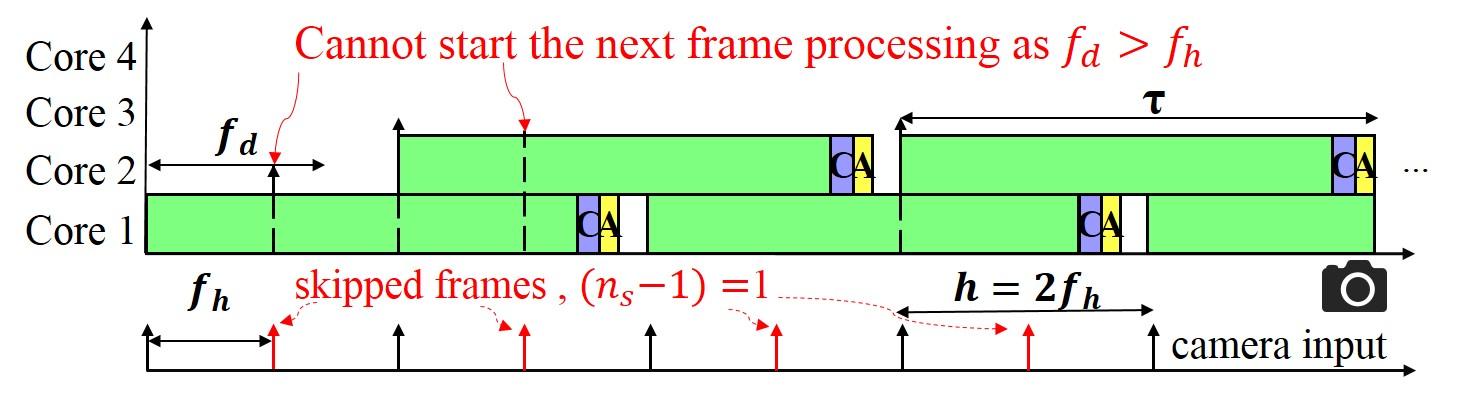
\includegraphics[width=\textwidth]{images/ifd.jpg}
    }
    \caption{Illustration of inter-frame dependencies with $\fh < \fd \le 2\fh$. (Adapted from Fig.~\ref{fig:ch6_ifd}, for readability.)}
    \label{fig:ch7_ifd}
    %\vspace{-2em}
\end{figure}
\subsubsection{Inter-frame dependencies in a pipelined implementation}
\label{sec:ch7_IFD}
Pipelining is inherently limited by inter-frame dependencies, i.e., the data or algorithmic dependencies between consecutive frame processing, e.g., due to video coding~\cite{li2015lagrangian} or visual tracking~\cite{smeulders2013visual}. 
Considering inter-frame dependencies is crucial for a practical pipelined implementation.
Inter-frame dependence time (denoted by $\fd$) can be quantified for the current image frame as the maximum time required to complete the processing of (parts of) the \gls{ibc} algorithm the subsequent image frame processing depends on. 
Alternatively, $\fd$ is the minimum time required to wait between the start of processing consecutive image frames.
Fig.~\ref{fig:ch7_ifd} illustrates the impact of inter-frame dependence time on sampling period $h$.
In a pipelined implementation, considering inter-frame dependencies means that strictly $h_{\mathit{eff}}\ge \fd$.
The number of frames that has to be skipped after processing every frame is $n_s-1$ with $n_s$ computed as in Step \ref{algoStep:ns} of Algorithm \ref{algo:SPADeFlow}. This is illustrated in Fig.~\ref{fig:ch7_ifd} where $n_s=2$ and one frame is skipped after every frame processing.

The computation of $\fd$ is explained in Algorithm~\ref{algo:SPADeFlow}. The inter-frame dependencies are modelled using the $\transformIFD$ model transformation explained in Section~\ref{sec:ch7_ModelTransformations}. Computing $\fd$ helps to determine the effective image arrival period or the minimum possible sampling period $h_{min}$ we can have.
Inter-frame dependencies mean that sometimes image frames have to be skipped for processing with respect to the given image arrival period $\fh$ and the sampling period $h$.
Skipping a frame means that $h$ increases and thus degrades the control performance.
In some cases, e.g., when the sensing uses video coding, inter-frame dependencies limit the effective camera frame rate and the video needs to be encoded/decoded at the effective rate $(1/h_{\mathit{eff}})$.
In case the video encoding is closed-source and the video encoding cannot be done at a new rate, then sufficient resources need to be allocated first for decoding at the original camera frame rate and only the remaining resources can be utilised for the rest of the application.
In this case, the video decoding is periodically executed at the camera frame rate and mapped first to the given platform allocation. The \gls{ibc} application is then mapped to the remaining allocation.

For a non-pipelined implementation, the inter-frame dependencies can be ignored since the frames are processed in sequence.

\begin{figure}[t]
\centerline{
    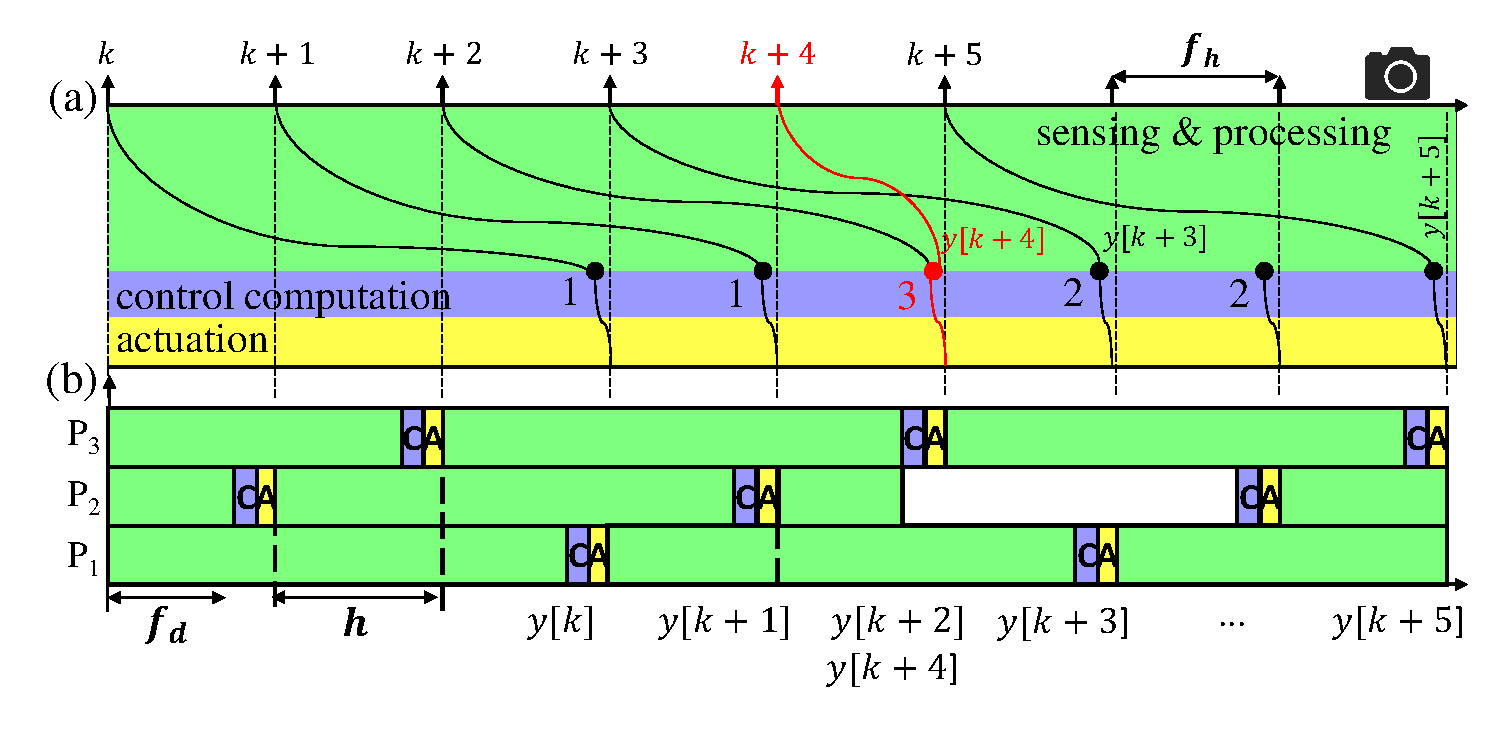
\includegraphics[width=\textwidth]{images/switching.eps}
    }
    \caption{Illustration of switching due to workload variations in a multiprocessor pipelined implementation. (a) Logical delay diagram  (adapted from Fig.~\ref{fig:ch6_pIBCvariations}) illustrating the cases explained in Sec~\ref{sec:ch7_switching_cases} and (b) its corresponding Gantt chart (adapted from Fig.~\ref{fig:ch6_pipelined_IBC}). The sample $k+4$ has a lower workload and thus the latest output measurement $y(k+4)$ is available within one $\fh$.}
    \label{fig:ch7_switching}
    %\vspace{-2em}
\end{figure}
\subsubsection{Switching in pipelined implementation}
\label{sec:ch7_switching_cases}
Switching in a multiprocessor pipelined \gls{ibc} system implementation due to workload variations has not been explicitly explored in literature apart from our previous work explained in Chapter~\ref{chap:pipelined}.
When we do not consider workload variations, a pipelined implementation effectively results in a constant $\tau$ and $h$.
Considering workload variations implies that we would have varying sensing delays, e.g. as illustrated in Fig.~\ref{fig:ch7_switching}. 
Here, notice that the camera input frame at $k+4$ has a sensing delay of one frame ($\tau_1=h$) due to lower image workload, and all other frames have a sensing delay of three frames ($\tau=3h$).
This scenario results in multiple sensing and image processing (\taskS) tasks completing their execution at the same time.
This means that multiple output measurements $y[k+2]$, and $y[k+4]$ are available for control computation task $\taskC$ at the same time instance.
For the scope of this work, the sampling period is kept constant and the switching happens due to variable delay.

Notice that by having just one frame with a lower workload, we can have the following three switching cases as illustrated in Fig.~\ref{fig:ch7_switching}~(a):
case~1) the new measurement is available with the same sensing delay as in the previous step; 
case~2) the sensing delay is increased compared to the previous step as the latest measurement is not available.
Older past measurements may be available during this time (e.g. $y[k+3]$ becomes available one period after $y[k+4]$). However, they are used only to update the state estimates and not directly for control input computation; 
case~3) the sensing delay is reduced by one or more steps: when multiple pipes finish processing a corresponding sequence of frames, both the latest measurement(s) along with the past measurements are now available.
The past measurements are used to update the state estimates, and the latest measurement is used to compute the control input.

Thus, the main challenge for the pipelined \gls{ibc} system design in order to maximise performance, i.e. \gls{qoc}, is to effectively use the sensor measurements as early as possible for control computation without any unnecessary idling and to estimate the system state when there are no sensor measurements available. Modelling this behaviour is far from trivial.
This problem was explored with respect to long network delays in~\cite{lincoln2000optimal}. We leverage these results in our design.

\begin{figure}[t]
\centerline{
    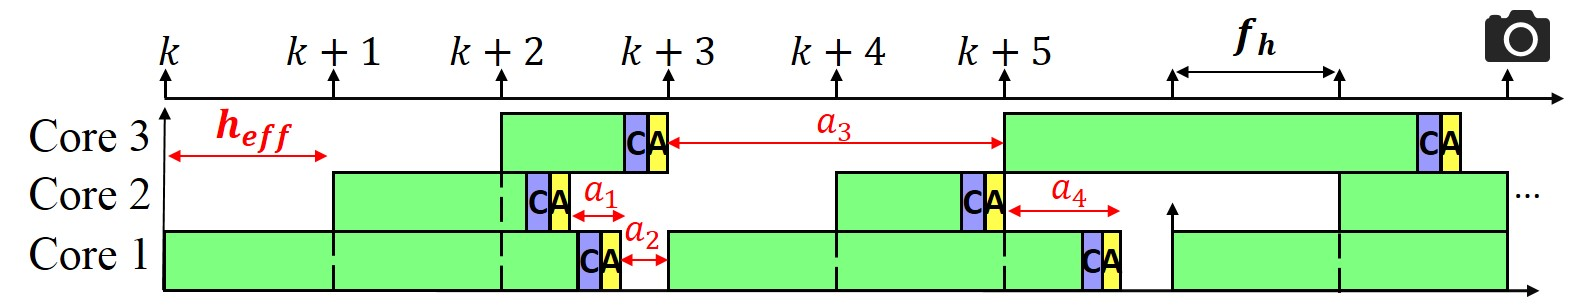
\includegraphics[width=\textwidth]{images/tau_dash_issue.jpg}
    }
    \caption{Illustration of the challenge with varying actuation rates $a_i$ due to variable $\tau_i^\prime$.}
    \label{fig:ch7_tau_dash_issue}
    %\vspace{-2em}
\end{figure}
\subsubsection{Control design and system-scenario identification}
\label{sec:ch7_controlDesignPipelined}
We consider a pipelined implementation with workload scenarios $\workloadScenario$ having $(\tau_i,\ h_i)$ as timing parameters.
It is possible to have a varying $h_i$ similar to the non-pipelined implementation.
However, proving stability guarantees then becomes challenging and as such is not explored in this work.
For the scope of this work, we assume a constant period $h_{\mathit{eff}}$ for all scenarios in the pipelined implementation.
How we compute $h_{\mathit{eff}}$ was explained earlier in Algorithm~\ref{algo:SPADeFlow}.
For brevity, $h=h_\mathit{eff}$ in the rest of this section.

For a workload scenario $\workloadScenario$, we can represent $\tau_i$ based on~\cite{ogata1995discrete} as
\begin{equation}
     \tau_i = (n_{f_i}-1)h+\tau_i^{\prime},\text{ where } 0<\tau_i^{\prime}\le h,\ n_{f_i}=\ceil[\bigg]{\frac{\tau_i}{h}}. \label{eq:ch7_tau_dash}
\end{equation}
This representation divides the delay $\tau_i$ into $n_{f_i}$ regions in the time domain.
This results in $(n_{f_i}-1)$ regions of $h$ and the left-over delay $\tau_i^\prime$ for $\tau_i$. 
$n_{f_i}$ is the number of frames arriving in one delay period for the scenario at hand. 
The above $n_{f_i}$ computation assumes the practical situation where $\tau_i>0$. 
In case one wants to consider $\tau_i=0$, $n_{f_i}=max\Big(\ceil[\Big]{\frac{\tau_i}{h}},1\Big)$.

Next, we enforce a constant actuation rate since a varying actuation rate results in undesired behaviour as illustrated in Fig.~\ref{fig:ch7_tau_dash_issue}, even in the case of a pipelined implementation with a constant sampling period.
Fig.~\ref{fig:ch7_tau_dash_issue} executes a scenario sequence $(s_3s_2s_1s_3s_1s_3)^\omega$ with sampling period $h_{\mathit{eff}}=\fh$. The scenario $s_1$ has the best-case delay $\tau_1=\fh$, $s_2$ has a delay $\tau_2=1.2\fh$, and $s_3$ has a delay $\tau_3=2.5\fh$. 
If we now apply Eq.~\ref{eq:ch7_tau_dash}, we get a varying $\tau_i^{\prime}$ and the Gantt chart as illustrated in Fig.~\ref{fig:ch7_tau_dash_issue}.
Notice that the actuation rates illustrated by the $a_i$
are not periodic anymore and we have ordering issues as well with respect to the actuation task. 
Further, guaranteeing controller stability for this case is challenging. 

We mitigate varying actuation rates by defining $\tau^{\prime}=\max \limits_i(\tau_i^{\prime})$ and then designing controllers with $\tau_i=(n_{f_i}-1)h+\tau^{\prime}$ and $h=h_{\mathit{eff}}$ for workload scenarios $\workloadScenario$. A constant $\tau^{\prime}$ over all scenarios is required to maintain a constant actuation rate between switching scenarios in a pipelined implementation. 
Notice that by defining and fixing $\tau^\prime$ we are aggregating workload scenarios with the same $n_{f_i}$ (see Eq.~\ref{eq:ch7_tau_dash}). The controllers are designed for these aggregated workload scenarios.
Also, the design space for system-scenario identification is narrowed down by the workload scenario aggregation.

To design the controllers, Eq.~\ref{eq:ch7_contsys} can then be reformulated as follows~\cite{ogata1995discrete}:
\begin{align}
\label{eq:ch7_sd_pipe}
x[k+1] = A_{\workloadScenario} x[k] &+ B_{0,\workloadScenario}^{\prime} u[k-(n_{f_i}-1)]\\  
                     &+ B_{1,\workloadScenario}^{\prime} u[k-n_{f_i}],\nonumber
\end{align}
where $A_{\workloadScenario},\ B_{0,\workloadScenario}^{\prime}$ and $B_{1,\workloadScenario}^{\prime}$ are given by replacing $\tau_i$ by $\tau^{\prime}$ and $h_i$ by $h$ in Eq.~\ref{eq:ch5_ch5_A_sk}.
It is interesting to note that the matrices $A_{\workloadScenario},\ B_{0,\workloadScenario}^{\prime}$ and $B_{1,\workloadScenario}^{\prime}$ are identical for all the scenarios due to this formulation.
However, Eq.~\ref{eq:ch7_sd_pipe} is still different for different aggregated scenarios due to varying $n_{f_i}$.
 We leverage the identical matrices during the runtime implementation as we only have to store a few key matrices as explained in Section~\ref{sec:ch7_implementation-aware control matrices}.
 
Next, we define new augmented system states $z^{\prime}[k]=\left[ \begin{array}{ccccc} x[k] &  u[k-(n_{f_i}-1)] & \cdots & u[k-2] & u[k-1] \end{array} \right]^T$ to obtain a higher-order augmented system as follows:
\begin{equation}
\label{eq:ch7_cld2_pipe}
z^{\prime}[k+1] = A_{\workloadScenario}^{\prime}z^{\prime}[k] + B_{\workloadScenario}^{\prime}u[k],\ 
y[k]=C^{\prime}z^{\prime}[k] + \Dcont u[k], \nonumber
\end{equation}
\begin{align}
%\begin{eqnarray}
A_{\workloadScenario}^{\prime} &= \left[ \begin{array}{ccccc} A_{\workloadScenario} &  B_{1,\workloadScenario}^{\prime} & B_{0,\workloadScenario}^{\prime} & \cdots & 0 \\  0 & 0 & I & \cdots & 0\\
\vdots & \vdots & \vdots & \ddots & \vdots\\
0 & 0 & 0 & \cdots & I\\
0 & 0 & 0 & \cdots & 0\\
\end{array} \right],\ 
B_{\workloadScenario}^{\prime} = \left[ \begin{array}{c} 0 \\ 0 \\ \vdots \\ 0 \\  I \end{array} \right],\nonumber\\
C^{\prime}&= \left[ \begin{array}{ccccc} \Ccont &  0 & 0 & \cdots & 0\end{array} \right].   
\label{eq:ch7_aug_pipe}
%\end{eqnarray}
\end{align}

Controllers are then designed for this higher-order augmented system, as explained in Section~\ref{sec:ch7_control_configuration}.
The stability criterion for the switched pipelined implementation is similar to the problem for long network delays~\cite{lincoln2000optimal,cloosterman2009stability} and as such is not explained here.

For the pipelined implementation, we identify system scenarios using the following steps, where the first two steps are done as part of the controller design:
i) classify the workload scenarios $\workloadScenario$ with the same $n_{f_i}=\ceil{\frac{\tau_{i}}{h}}$ into a maximum of $\ceil{\frac{\tau_{wc}}{\fh}}$ aggregated workload scenarios; 
ii) for each aggregated workload scenario, design a controller with $\tau_i=(n_{f_i}-1)h+\tau^{\prime}$ and $h=h_{\mathit{eff}}$; 
iii) check for control stability for the switched system with the identified aggregated workload scenarios. If the switched system is unstable, find an aggregation of workload scenarios for which the switched system is stable through an exhaustive search. If multiple scenario sets provide a stable system, we choose the set with the highest cardinality and shortest average sensor-to-actuator delay; 
iv) the identified aggregated workload scenarios that result in a stable switched system are the system scenarios $\sysScenario$ with $\tau_s=(n_{f_s}-1)h+\tau^{\prime}$ and $h=h_{\mathit{eff}}$.

\subsubsection{Implementation-aware control matrices and control configurations}
\label{sec:ch7_implementation-aware control matrices}
When we allow switching for pipelined implementation, the challenge is the varying dimensions of matrices in Eq.~\ref{eq:ch7_aug_pipe} for varying delays due to workload variations.
The varying dimensions affect the runtime computation of $u[k]$ (see Eq.~\ref{eqn:u}), where the matrix $\Kgain_i$ needs to be multiplied with $z[k]$ at every time-step. 
This challenge also occurs when some of the system states are estimated and not directly obtained from sensor measurements. For the \gls{lkas}, only the third state is computed from the sensor and the other states are estimated using the system model (see Eq.~\ref{eq:ch7_cld2}).
In this case, $z[k+1]$ (see Eq.~\ref{eq:ch7_cld2}) needs to be computed at every time step.

We tackle the challenge of varying dimensions of matrices by unifying/normalising the dimensions of matrices considering the worst-case delay $\tau_{wc}$ over all system scenarios $\sysScenario$. 
The matrices for the worst-case delay scenario $s_{wc}$ annotated with $(h,\tau_{wc})$ are the same as in Eq.~\ref{eq:ch7_aug_pipe}. 
Let $n$ be the order of the square matrix $A_{s_{wc}}$ and $n_{f_{wc}}=\ceil{\frac{\tau_{wc}}{h}}$.
For each system scenario $\sysScenario$, with $\tau_s > h$,
$n_{f_s}=\ceil{\frac{\tau_{s}}{h}}$, the system matrices are given below. For brevity, let $n_{f_{wc}}=n_f$ and $n$ is the order of matrix $A_{\sysScenario}$.
It is interesting to note that $A_{\sysScenario}=A_{s_{wc}}$ when the period $h$ is constant for the system scenarios $\sysScenario$.
The order of the square matrix $A_{\sysScenario}^{\prime}$ is ($n+n_f$).

\begin{align}
A_{\sysScenario}^{\prime} &= \left[ 
\begin{array}{lcc} 
A_{\sysScenario} & 0_{(n_{f}-1)\times n} & 0_{1\times n}\\
0_{n\times (n_{f}-n_{f_s})} &  & \\
B_{1,\sysScenario}^{\prime} & 0_{(n_{f}-1)\times 1} & 0_{1\times 1}\\
B_{0,\sysScenario}^{\prime} & & \\
0_{n\times (n_{f_s}-2)} & I_{(n_{f}-1)\times (n_{f}-1)} & 0_{1\times (n_{f}-1)}\\
\end{array}
\right]^T,\nonumber\\ 
B_{\sysScenario}^{\prime} &= \left[ \begin{array}{cc} 0_{(n+n_{f}-1) \times 1} & I_{1\times 1} \end{array} \right]^T,\ 
C^{\prime}= \left[ \begin{array}{cc} \Ccont &  0_{1\times n_{f}}
\end{array}
\right].  \nonumber  
%\label{eq:ch7_aug_implement}
\end{align}

Further, in a pipelined implementation due to workload variations we could have a scenario $\sysScenario$ with $\tau_s\le h$ (see for instance iteration $[k+4]$ in Fig.~\ref{fig:ch7_switching}). We derive the matrices for such scenarios as follows. 
Also, since $\tau_s\le h$, $n_{f_s}=1$.
\begin{align}
A_{\sysScenario}^{\prime} &= \left[ \begin{array}{lll} A_{\sysScenario} &  0_{n\times (n_{f}-n_{f_{s}})} & B_{1,\sysScenario}^{\prime} \\  
0_{(n_{f}-1)\times n} & 0_{(n_{f}-1)\times 1}  & I_{(n_{f}-1)\times (n_{f}-1)} \\
0_{1\times n} & 0_{1\times 1} & 0_{1\times (n_{f}-1)}\\
\end{array} \right],\nonumber\\ 
B_{\sysScenario}^{\prime} &= \left[ \begin{array}{ccc} B_{0,\sysScenario}^{\prime} & 0_{(n_{f}-1) \times 1} & I_{1\times 1} \end{array} \right]^T,\nonumber\\ 
C^{\prime} &= \left[ \begin{array}{cc} \Ccont &  0_{1\times n_{f}}\end{array} \right].  \nonumber  
\end{align}

The matrices $A_{\sysScenario},\ B_{0,\sysScenario}^{\prime}$ and $B_{1,\sysScenario}^{\prime}$ are obtained for scenario $\sysScenario$ as explained in Eq.~\ref{eq:ch7_aug_pipe}.
We can apply standard control design techniques for these implementation-aware system models.
State-feedback and feed-forward controllers can be designed as shown in Eq.~\ref{eqn:u} for the system scenarios to obtain $\Kgain_s$ and $\Fgain_s$.
The control configurations are then $\Configuration_{\sysScenario}^c = (h_{\mathit{eff}},\tau_{s}, \Kgain_{s}, \Fgain_{s})$.

Note that when storing matrices for a pipelined implementation, we only need to store $\Kgain_s$ and $\Fgain_s$ for each scenario $\sysScenario$, $A_{s_{wc}}$, $B_{0,\sysScenario}^{\prime}$, $B_{1,\sysScenario}^{\prime}$, and $\Ccont$ for the constant period $h$ and $\tau^\prime$. We only need to store one $A_{s_{wc}}$, $B_{0,\sysScenario}^{\prime}$, $B_{1,\sysScenario}^{\prime}$, and $\Ccont$ matrix as the period and actuation rate are constant. 